\chapter{Conception des PCB}

Afin de réaliser le circuit imprimé de notre projet, nous avons utilisé le logiciel de conception de PCB \textit{Proteus}, dans lequel nous avons reproduit le schéma électrique complet vu précédemment.
Cependant, pour faciliter la réalisation du PCB, nous avons dû apporter quelques modifications au schéma initial pour bien préparer la carte à la fabrication et à l'assemblage. Pour cela, nous avons créer les différents empreintes des composants utilisés, en veillant à respecter les dimensions réelles de chaque composant, données par les fiches techniques des fabricants. Nous avons également pensé à définir les zones de cuivre pour l'alimentation et la masse (plan de masse), afin de faciliter le routage et d'améliorer les performances électriques de la carte. Enfin, nous avons ajouté des perçages pour les fixations mécaniques de la carte dans son boîtier.

\begin{figure}[H]
    \centering
    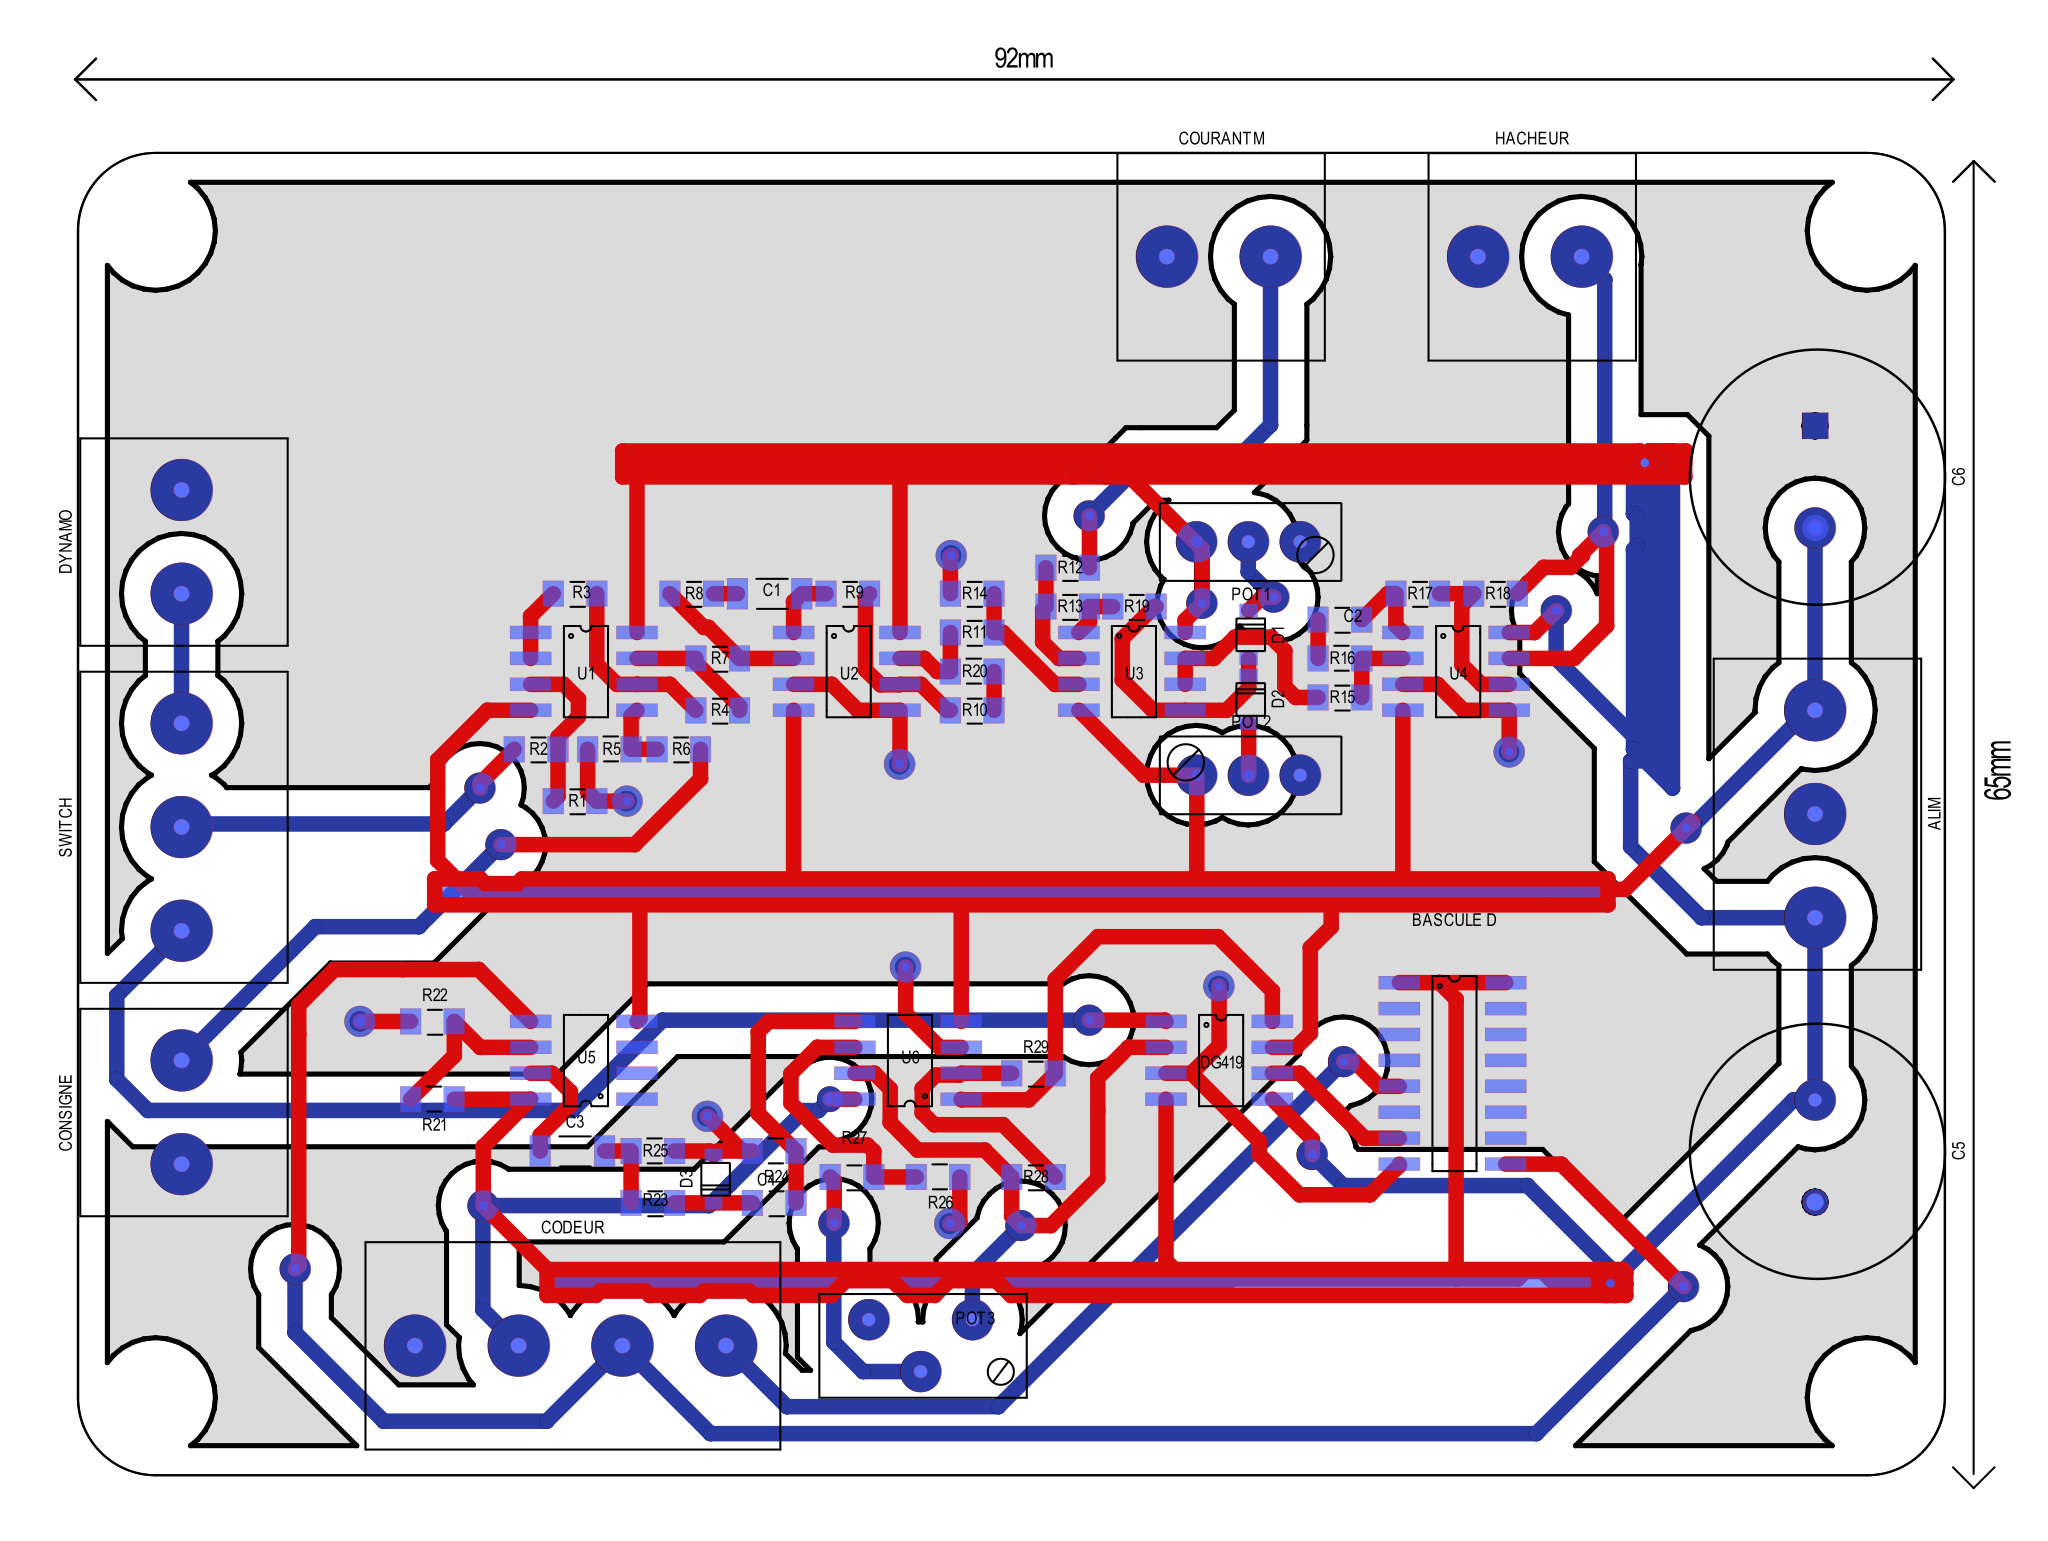
\includegraphics[width=0.8\textwidth]{images/Image PCB/Carte_PCB.pdf}
    \caption{Schéma de la conception du PCB}
    \label{fig:pcb_design}
\end{figure}
\figref{Figure \ref{fig:pcb_design}}{Modélisation\_Finale\_VALIDE\_13\_01\_2026/07\_Conception\_PCB/PCB\_Final\_ProjetGES7\_2025\_27\_11.pdsprj}

Concernant le placement des composants sur le PCB, nous avons répartis les composants sur deux "étages". Le premier étage (celui du haut sur l'image \ref{fig:pcb_design}) comporte toute la chaine d'asservissement du moteur en courant et en vitesse. Tandis que le second étage (celui du bas sur l'image \ref{fig:pcb_design}) contient les composants liés au traitement du signal de sortie du codeur incrémental.


\newpage
En ce qui concerne le connecteur VGA, nous avons également conçu son PCB et son schéma électrique dans \textit{Proteus}, en respectant le standard de câblage VGA prescrit sur Moodle pour assurer une bonne compatibilité avec l'équipement que nous utilisons.

\begin{figure}[H]
    \centering
    \begin{subfigure}[t]{0.48\textwidth}
        \centering
        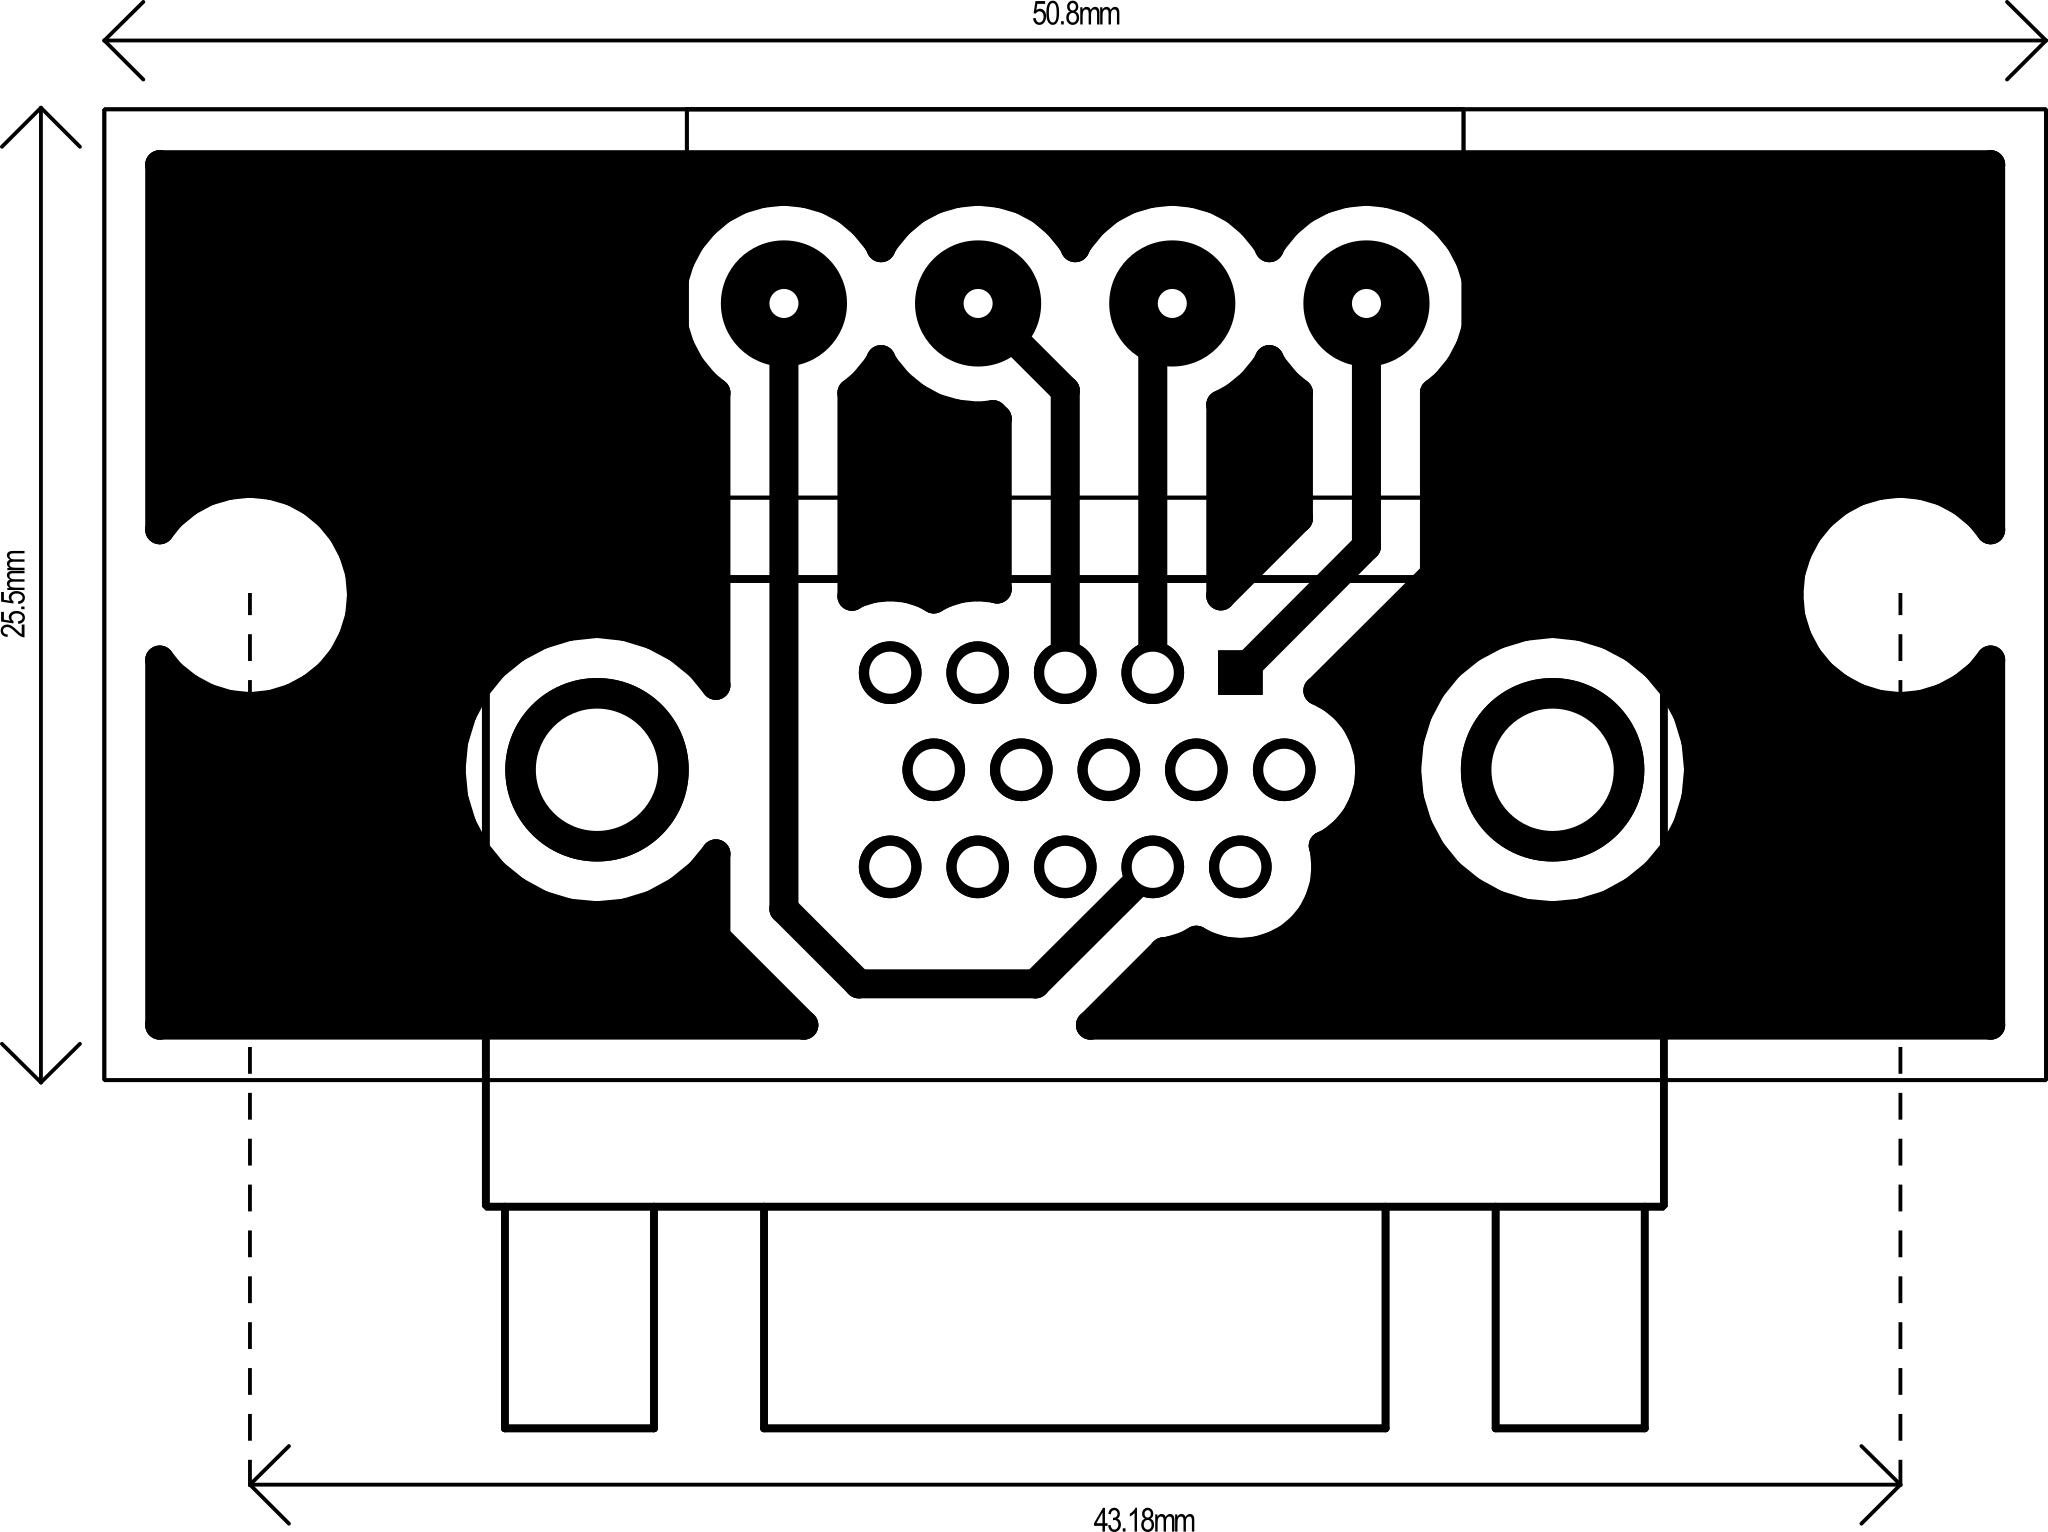
\includegraphics[width=\textwidth]{images/Image PCB/VGA_PCB.pdf}
        \caption{PCB du connecteur VGA}
    \end{subfigure}
    \hfill
    \begin{subfigure}[t]{0.35\textwidth}
        \centering
        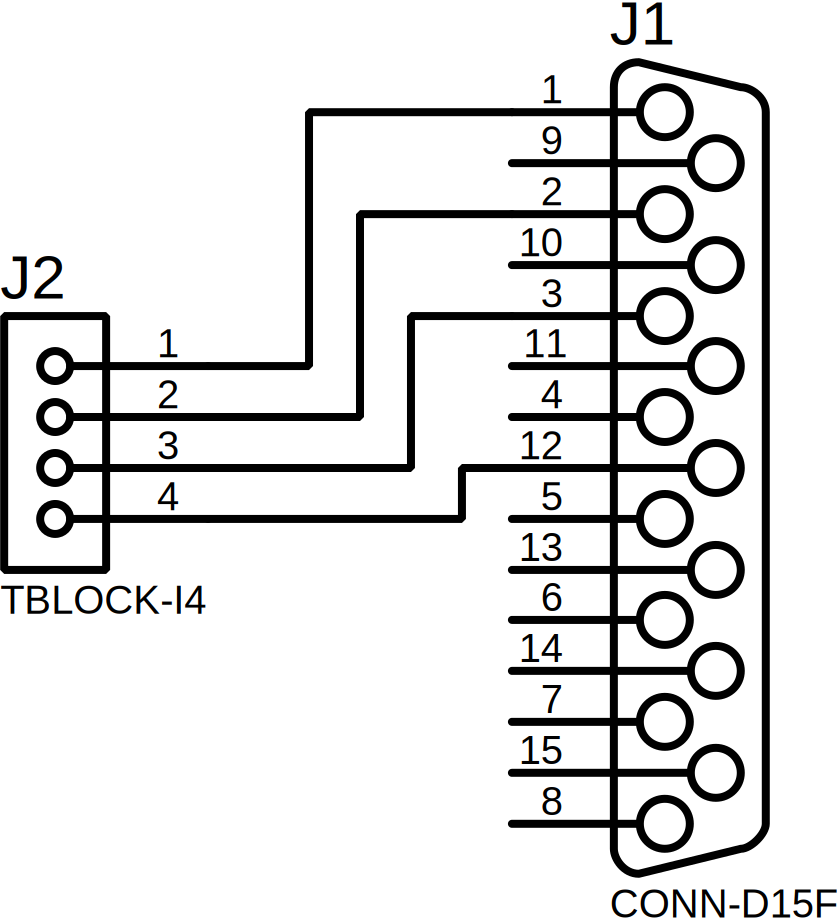
\includegraphics[width=\textwidth]{images/Image PCB/VGA_SCHEMA.pdf}
        \caption{Schéma du connecteur VGA}
    \end{subfigure}
    \caption{Conception du connecteur VGA}
    \label{fig:vga_design}
\end{figure}
\figref{Figure \ref{fig:vga_design}}{Modélisation\_Finale\_VALIDE\_13\_01\_2026/07\_Conception\_PCB/Carte VGA.pdsprj}